\makeatletter
\pgfdeclareshape{document}{
	\inheritsavedanchors[from=rectangle] % this is nearly a rectangle
	\inheritanchorborder[from=rectangle]
	\inheritanchor[from=rectangle]{center}
	\inheritanchor[from=rectangle]{north}
	\inheritanchor[from=rectangle]{south}
	\inheritanchor[from=rectangle]{west}
	\inheritanchor[from=rectangle]{east}
	% ... and possibly more
	\backgroundpath{% this is new
		% store lower right in xa/ya and upper right in xb/yb
		\southwest \pgf@xa=\pgf@x \pgf@ya=\pgf@y
		\northeast \pgf@xb=\pgf@x \pgf@yb=\pgf@y
		% compute corner of ‘‘flipped page’’
		\pgf@xc=\pgf@xb \advance\pgf@xc by-10pt % this should be a parameter
		\pgf@yc=\pgf@yb \advance\pgf@yc by-10pt
		% construct main path
		\pgfpathmoveto{\pgfpoint{\pgf@xa}{\pgf@ya}}
		\pgfpathlineto{\pgfpoint{\pgf@xa}{\pgf@yb}}
		\pgfpathlineto{\pgfpoint{\pgf@xc}{\pgf@yb}}
		\pgfpathlineto{\pgfpoint{\pgf@xb}{\pgf@yc}}
		\pgfpathlineto{\pgfpoint{\pgf@xb}{\pgf@ya}}
		\pgfpathclose
		% add little corner
		\pgfpathmoveto{\pgfpoint{\pgf@xc}{\pgf@yb}}
		\pgfpathlineto{\pgfpoint{\pgf@xc}{\pgf@yc}}
		\pgfpathlineto{\pgfpoint{\pgf@xb}{\pgf@yc}}
		\pgfpathlineto{\pgfpoint{\pgf@xc}{\pgf@yc}}
	}
}
\makeatother

\newcommand\myfigureSystemArchitecture{
	\beginpgfgraphicnamed{systemarchitecture}
	\begin{tikzpicture}[%
		remember picture,
		text centered,
		start chain,
		node distance=1cm,
		every on chain/.style={join=by ->},
		every join/.style={line width=1.25pt}]
		\tikzstyle{unit} = [line width=1.0pt, auto]
		\tikzstyle{model} = [line width=1.0pt, auto, text width=2cm]
		\tikzstyle{line} = [draw, line width=1.25pt, join=by ->]
		\matrix (m) [matrix of nodes, 
		column sep=7.2mm,
		row sep=12mm,
		inner sep=3pt,
		nodes={draw, % General options for all nodes
		  line width=0.7pt,
		  anchor=center, 
		  text centered
		},
		bases/.style={
			minimum width=1.6cm, 
			text width=1.6cm, 
			tape
		},
		doc/.style={
			tape,
			text width=1.5cm, 
			minimum width=1.5cm,
			minimum height=9mm
		},
		docs/.style={
			tape,
			copy shadow,
			fill=white,
			text width=1.5cm, 
			minimum width=2cm,
			minimum height=11mm
		},
		sets/.style={
			copy shadow,
			fill=white,
			text width=1.25cm, 
			minimum width=1.5cm
		},
		subsystem/.style={
			line width=1.25pt,
			text width=1.9cm, 
			minimum width=1cm,
			minimum height=9mm
		},
		system/.style={
			line width=1.25pt,
			text width=1.9cm, 
			minimum width=2.1cm,
			minimum height=9mm
		},
		source/.style={
			shadow xshift=1ex,
			shadow yshift=1ex,
			cylinder,
			fill=white,
			shape border rotate=90,
			shape aspect=.1,
			line width=1.25pt,
			text width=1.5cm, 
			minimum width=1cm,
			minimum height=11mm
		},
		hexprog/.style={
			document,
			fill=white,
			text width=1.6cm, 
			minimum width=1.2cm,
			minimum height=12mm
		},
		sources/.style={
			shadow xshift=1ex,
			shadow yshift=1ex,
			cylinder,
			copy shadow,
			fill=white,
			shape border rotate=90,
			shape aspect=.1,
			line width=1.25pt,
			text width=1.5cm, 
			minimum width=1cm,
			minimum height=11mm
		}
		]
		{
			|[hexprog]| \hex-Program	\pgfmatrixnextcell |[subsystem]| Evaluation Framework	\pgfmatrixnextcell \pgfmatrixnextcell \pgfmatrixnextcell |[docs]| Answer Sets \\
						\pgfmatrixnextcell |[subsystem]| Model Generators \pgfmatrixnextcell \pgfmatrixnextcell \pgfmatrixnextcell |[system]| ASP Solver   \\
			|[system]| ASP Grounder	\pgfmatrixnextcell |[subsystem]| \hex{}-Grounder		\pgfmatrixnextcell |[subsystem]| Post Propagator \pgfmatrixnextcell |[subsystem]| UFS-Checker \pgfmatrixnextcell |[system]| SAT Solver   \\
						\pgfmatrixnextcell  \pgfmatrixnextcell  |[sources]| Plugins \pgfmatrixnextcell \pgfmatrixnextcell  \\
		};
		%
		\draw[dashed] ($(m-1-2)+(-1.5cm,+1.0cm)$) rectangle node [xshift=3.2cm,yshift=3.35cm] {\dlvhex{} core} ($(m-3-4)+(1.5cm,-0.7cm)$);
		\path[draw,line width=1pt,->] (m-1-1) -- node [scale=0.5,shape=circle,draw,fill=white] {1} (m-1-2);
		\path[draw,line width=1pt,<->] (m-1-2) -- node [scale=0.5,shape=circle,draw,fill=white] {2} (m-2-2);
		\path[draw,line width=1pt,<->] (m-2-2) -- node [scale=0.5,shape=circle,draw,fill=white] {3} (m-3-2);
		\path[draw,line width=1pt,<->] (m-3-2) -- node [scale=0.5,shape=circle,draw,fill=white] {4} (m-3-1);
		\path[draw,line width=1pt,<->] (m-3-2) -- node [scale=0.5,shape=circle,draw,fill=white] {5} (m-4-3);
		\path[draw,line width=1pt,<->] (m-2-2) -- node [scale=0.5,shape=circle,draw,fill=white] {6} (m-2-5);
		\path[draw,line width=1pt,<->] (m-2-5) -- node [scale=0.5,shape=circle,draw,fill=white] {7} (m-3-3);
		\path[draw,line width=1pt,<->] (m-3-3) -- node [scale=0.5,shape=circle,draw,fill=white] {8} (m-3-4);
		\path[draw,line width=1pt,<->] (m-3-3) -- node [scale=0.5,shape=circle,draw,fill=white] {9} (m-4-3);
		\path[draw,line width=1pt,<->] (m-3-4) -- node [scale=0.5,shape=circle,draw,fill=white] {10} (m-4-3);
		\path[draw,line width=1pt,<->] (m-3-4) -- node [scale=0.5,shape=circle,draw,fill=white] {11} (m-3-5);
		\path[draw,line width=1pt,->] (m-1-2) -- node [scale=0.5,shape=circle,draw,fill=white] {12} (m-1-5);
	\end{tikzpicture}
	\endpgfgraphicnamed
}
%
\newcommand\myfigureTikzAtomDepGraph{%
    \beginpgfgraphicnamed{atomdepgraph}%
    \small%
    \begin{tikzpicture}%[inner ysep=0.15em]%
    \begin{scope}[xscale=3,yscale=-1.7]
      \node (swimin) at (1,1) {$\mygoinout(\myindoor)$};
      \node (swimout) at (2,1) {$\mygoinout(\myoutdoor)$};
      \node (rqswim) at (1,2) {$\ext{\mycost}{\mygoinout}{C}$};
      \node (swimp) at (2,2) {$\mygoinout(P)$};
      \node (needinout) at (0.5,3) {$\myneed(\myinout,C)$};
      \node (gotox) at (1.5,3) {$\mygolocation(X)$};
      \node (ngotox) at (2.5,3) {$\myngolocation(X)$};
      \node (gotoy) at (2.5,4.5) {$\mygolocation(Y)$};
      \node (go) at (2,4.5) {$\mygosomewhere$};
      \node (rqgoto) at (1.25,3.75) {$\ext{\mycost}{\mygolocation}{C}$};
      \node (needloc) at (1.25,4.5) {$\myneed(\mygolocation,C)$};
      \node (needmoney) at (0.5,5.0) {$\myneed(X,\mymoney)$};
    \end{scope}
    \begin{scope}
      \draw (swimin.south east) edge[bend right,->] node[midway,above] {$_m$} (swimout.south west);
      \draw (swimout.north west) edge[bend right,->] node[midway,above] {$_m$} (swimin.north east);
      \draw (rqswim.north) edge[->] node[midway,left] {$^e_m\!$} (swimin);
      \draw (rqswim.north east) edge[->] node[near end,below] {$^e_m$} (swimout);
      \draw (swimp.north) edge[->] node[midway,right] {$_m$} (swimout);
      \draw (swimp.north west) edge[->] node[near end,below] {$_m$} (swimin);
      \draw (needinout.north) edge[->] node[midway,left] {$_m$} (rqswim);
      \draw (gotox.north) edge[->] node[midway,left] {$_m$} (swimp);
      \draw (ngotox.north) edge[->] node[midway,left] {$_m$} (swimp);
      \draw (gotox.south east) edge[bend right,->] node[midway,above] {$_m$} (ngotox.south west);
      \draw (ngotox.north west) edge[bend right,->] node[midway,above] {$_m$} (gotox.north east);
      \draw (gotox.north west) edge[bend left=-115,distance=10mm,->] node[midway,right] {$_m$} (gotox.south west);

      \draw (rqgoto.north) edge[->] node[midway,left] {$^e_m$} (gotox);

      \draw (needloc.north) edge[->] node[midway,left] {$_m$} (rqgoto);
      \draw (gotoy.north) edge[->] node[midway,right] {$_m$} (gotox);
      \draw (go.north) edge[->] node[midway,right] {$_m$} (gotox);

      \draw (needmoney) edge[->] node[midway,left] {$_m$} (needinout);
      \draw (needmoney) edge[->] node[near end,below] {~$_m$} (needloc);
    \end{scope}
    \end{tikzpicture}%
    \endpgfgraphicnamed%
}%\myfigureTikzAtomDepGraph
%
\newcommand\myfigureTikzRuleDepGraph{%
    \beginpgfgraphicnamed{ruledepgraph}%
    \small%
    \begin{tikzpicture}%[inner ysep=0.15em]%
    \begin{scope}[xscale=3,yscale=-1.5]
      \node (r1) at (2,1)
        {$r_1{:}\ \mygoinout(\myindoor) \lors \mygoinout(\myoutdoor) \lif$};
      \node (r2) at (1,2)
        {$\begin{array}{@{}l@{}}
            r_2{:}\ \myneed(\myinout,C) \lifs \\
            \qquad\quad\ext{\mycost}{\mygoinout}{C}
          \end{array}$};
      \node (r3) at (3,2)
        {$\begin{array}{@{}l@{}}
            r_3{:}\ \mygolocation(X) \lors \myngolocation(X) \lifs\\
            \qquad\quad\mygoinout(P), \mylocation(P,X)
          \end{array}$};
      \node (r4) at (3.75,3)
        {$r_4{:}\ \mygosomewhere \lifs \mygolocation(X)$};
      \node (r5) at (1.75,3)
        {$\begin{array}{@{}l@{}}
            r_5{:}\ \myneed(\myloc,C) \lifs \\
            \qquad\quad\ext{\mycost}{\mygolocation}{C}
          \end{array}$};
      \node (c6) at (2.5,4)
        {$c_6{:}\ \lifs \mygolocation(X), \mygolocation(Y), X\,{\neq}\,Y$};
      \node (c7) at (3.75,4)
        {$c_7{:}\ \lifs \naf \mygosomewhere$};
      \node (c8) at (1,4)
        {$c_8{:}\ \lifs \myneed(X,\mymoney)$};
    \end{scope}
    \begin{scope}
      \draw (r2) edge[->] node[midway,above] {$_m$} (r1);
      \draw (r3) edge[->] node[midway,above] {$_m$} (r1);

      \draw (r5) edge[->] node[midway,above] {$_m$} (r3);
      \draw (r4) edge[->] node[midway,right] {$\ _m$} (r3);

      \draw (c6) edge[->] node[midway,left] {$_m$} (r3);
      \draw (c7) edge[->] node[midway,right] {$_{\mi{nm}}$} (r4);
      \draw (c8) edge[->] node[midway,left] {$_m$} (r2);
      \draw (c8) edge[->] node[midway,right] {$\ _m$} (r5);
    \end{scope}
    \end{tikzpicture}%
    \endpgfgraphicnamed%
}%\myfigureTikzAtomDepGraph
%
\newcommand\myfigureExOldEvalStrat{%
    \beginpgfgraphicnamed{exOldEvalStrat}%
    \small%
    \begin{tikzpicture}[inner ysep=0.15em]%
    \node[rectangle,draw,inner xsep=0.20em] (comp1) at (0,4)
      {$\begin{array}{@{}l@{}}
      r_1{:}\;\mygoinout(\myindoor) \lors \mygoinout(\myoutdoor) \lifs. \\
      r_3{:}\;\mygolocation(X) \lors \myngolocation(X) \lifs
      \mygoinout(P), \mylocation(P,X). \\
      r_4{:}\;\mygosomewhere \lifs \mygolocation(X). \\
      c_6{:}\;{\lif}\, \mygolocation(X), \mygolocation(Y), X \neq Y. \\
      c_7{:}\;{\lif}\, \naf \mygosomewhere. \\
      \text{derives: } \mygoinout(X),\;
                       \mygolocation(X),\;
                       \myngolocation(X),\;
                       \mygosomewhere
      \end{array}$};
    \node[rectangle,draw,below=4mm of comp1,inner xsep=0.2em] (comp2)
      {$\begin{array}{@{}l@{}}
      r_2{:}\;\myneed(\myinout,C) \lifs \ext{\mycost}{\mygoinout}{C}. \\
      r_5{:}\;\myneed(\myloc,C) \lifs \ext{\mycost}{\mygolocation}{C}. \\
      \text{derives: } \myneed(A,B)
      \end{array}$};
    \node[rectangle,draw,below=4mm of comp2] (comp3)
      {$\begin{array}{@{}l@{}}
      c_8{:}\;{\lif}\, \myneed(X,\mymoney). \\
      \text{derives nothing}
      \end{array}$};
    \node[anchor=east,inner sep=0pt,outer sep=0pt] at (comp1.west) {$u_1\,$};
    \node[anchor=east,inner sep=0pt,outer sep=0pt] at (comp2.west) {$u_2\,$};
    \node[anchor=east,inner sep=0pt,outer sep=0pt] at (comp3.west) {$u_3\,$};
    \draw[->] (comp2.north) -- (comp1.south);
    \draw[->] (comp3.north) -- (comp2.south);
    \end{tikzpicture}%
    \endpgfgraphicnamed%
}% \newcommand\myfigureExOldEvalStrat{%
%
\newcommand\myfigureExOldEvalModel{%
    \beginpgfgraphicnamed{exOldEvalModel}%
    \small%
    \begin{tikzpicture}[inner ysep=0.2em,inner xsep=0.2em]%
    \begin{scope}[xscale=3.0,yscale=-1.5]
    % input u1
    \node[rectangle,draw] (m1) at (2.5,0.75) {$\emptyset$};
      \node[anchor=south] (m1label) at (m1.north) {$m_1/\scI$};
    % outputs u1
    \node[rectangle,draw] (m2) at (0.9,2) {
      $\begin{array}{@{}r@{}l@{}}
        \{ & \mygoinout(\myindoor), \mygosomewhere, \\
           & \myngolocation(\mypoola), \\
           & \mygolocation(\mypoolm) \} \end{array}$};
      \node[anchor=south east] at (m2.north) {$m_2/\scO$};
    \node[rectangle,draw] (m3) at (2.1,2) {
      $\begin{array}{@{}r@{}l@{}}
        \{ & \mygoinout(\myindoor), \mygosomewhere, \\
           & \myngolocation(\mypoolm), \\
           & \mygolocation(\mypoola) \} \end{array}$};
      \node[anchor=south east] at (m3.north) {$m_3/\scO$};
    \node[rectangle,draw] (m4) at (3.295,2) {
      $\begin{array}{@{}r@{}l@{}}
        \{ & \mygoinout(\myoutdoor), \mygosomewhere, \\
           & \myngolocation(\mypoolg), \\
           & \mygolocation(\mypooln) \} \end{array}$};
      \node[anchor=south west] at (m4.north) {$m_4/\scO$};
    \node[rectangle,draw] (m5) at (4.42,2) {
      $\begin{array}{@{}r@{}l@{}}
        \{ & \mygoinout(\myoutdoor), \mygosomewhere, \\
           & \myngolocation(\mypooln), \\
           & \mygolocation(\mypoolg) \} \end{array}$};
      \node[anchor=south west] at (m5.north) {$m_5/\scO$};
    %
    % inputs u2
    \node[rectangle,draw,below=11mm of m2] (m6) {
      $\myint(m_2)$};
      \node[anchor=south west] (m6label) at (m6.north) {$\,m_6/\scI$};
    \node[rectangle,draw,below=11mm of m3] (m7) {
      $\myint(m_3)$};
      \node[anchor=south] at (m7.north west) {$m_7/\scI$};
    \node[rectangle,draw,below=11mm of m4] (m8) {
      $\myint(m_4)$};
      \node[anchor=south] at (m8.north west) {$m_8/\scI$};
    \node[rectangle,draw,below=11mm of m5] (m9) {
      $\myint(m_9)$};
      \node[anchor=south] at (m9.north west) {$m_9/\scI$};
    % outputs u2
    \node[rectangle,draw,below=7mm of m6] (m10) {
      $\begin{array}{@{}r@{}l@{}}
        \{ & \myneed(\myinout, \mymoney) \} \\
        \end{array}$};
      \node[anchor=south west] at (m10.north west) {$\,m_{10}/\scO$};
    \node[rectangle,draw,below=7mm of m7] (m11) {
      $\begin{array}{@{}r@{}l@{}}
        \{ & \myneed(\myinout,\mymoney), \\
           & \myneed(\myloc,\mygoggles) \} \end{array}$};
      \node[anchor=south west] at (m11.north west) {$m_{11}/\scO$};
    \node[rectangle,draw,below=7mm of m8] (m12) {
      $\begin{array}{@{}r@{}l@{}}
        \{ & \myneed(\myloc, \myyogamat) \} \\
        \end{array}$};
      \node[anchor=south west] at (m12.north west) {$m_{12}/\scO$};
    \node[rectangle,draw,below=7mm of m9] (m13) {
      $\begin{array}{@{}r@{}l@{}}
        \{ & \myneed(\myloc, \mymoney) \} \\
        \end{array}$};
      \node[anchor=south west] at (m13.north west) {$m_{13}/\scO$};
    %
    % inputs u3
    \node[rectangle,draw,below=20mm of m10.north] (m14) {
      $\myint(m_{10})$};
      \node[anchor=south west] (m14label) at (m14.north) {$\,m_{14}/\scI$};
    \node[rectangle,draw,below=20mm of m11.north] (m15) {
      $\myint(m_{11})$};
      \node[anchor=south] at (m15.north west) {$m_{15}/\scI$};
    \node[rectangle,draw,below=20mm of m12.north] (m16) {
      $\myint(m_{12})$};
      \node[anchor=south] at (m16.north west) {$m_{16}/\scI$};
    \node[rectangle,draw,below=20mm of m13.north] (m17) {
      $\myint(m_{13})$};
      \node[anchor=south] at (m17.north west) {$m_{17}/\scI$};
    % u2 outputs
    \node[below=5mm of m14] (m14no) {\Lightning};
    \node[below=5mm of m15] (m15no) {\Lightning};
    \node[rectangle,draw,below=5mm of m16] (m18)
      {$\emptyset$};
      \node[anchor=east] at (m18.west) {$m_{18}/\scO\,$};
    \node[below=5mm of m17] (m17no) {\Lightning};
    \end{scope}
    %
    % dependencies
    \begin{scope}[->]
    \draw (m2.north) -- (m1);
    \draw (m3) -- (m1);
    \draw (m4) -- (m1);
    \draw (m5.north) -- (m1);
    %
    \draw (m6) -- (m2);
    \draw (m7) -- (m3);
    \draw (m8) -- (m4);
    \draw (m9) -- (m5);
    %
    \draw (m10) -- (m6);
    \draw (m11) -- (m7);
    \draw (m12) -- (m8);
    \draw (m13) -- (m9);
    %
    \draw (m14) -- (m10);
    \draw (m15) -- (m11);
    \draw (m16) -- (m12);
    \draw (m17) -- (m13);
    %
    \draw (m14no) -- (m14);
    \draw (m15no) -- (m15);
    \draw (m18) -- (m16);
    \draw (m17no) -- (m17);
    \end{scope}
    %
    \node[rectangle,draw,inner sep=0.5em,
      fit=(m1) (m1label) (m2) (m5)] (u1) {};
      \node[left=0mm of u1] {\rotatebox{90}{at unit $u_1$}};
    \node[rectangle,draw,inner sep=0.5em,
      fit=(m6) (m6label) (m9) (m10) (m11) (m13)] (u2) {};
      \node[left=0mm of u2,outer sep=0,inner sep=0] {\rotatebox{90}{at unit $u_2{\big.}$}};
    \node[rectangle,draw,inner sep=0.5em,
      fit=(m14) (m14label) (m17) (m14no) (m17no)] (u3) {};
      \node[left=0mm of u3] {\rotatebox{90}{at unit $u_3$}};
    \end{tikzpicture}%
    \endpgfgraphicnamed%
}%\myfigureExOldEvalModel
%
\newcommand\myfigureExBetterEvalStrat{%
    \beginpgfgraphicnamed{exBetterEvalStrat}%
    \small%
    \begin{tikzpicture}[inner ysep=0.25em,xscale=1.5,yscale=1.2]%
      \node[rectangle,draw] (comp1) at (0.5,4.8)
        {$\begin{array}{@{}l@{}}
          r_1{:}\;\mygoinout(\myindoor) \lors \mygoinout(\myoutdoor) \,{\lif}. \\
          \text{derives: } \mygoinout(X)
        \end{array}$};
      \node[rectangle,draw,inner xsep=0.2em,anchor=east] (comp2) at (0.2,3)
        {$\begin{array}{@{}l@{}}
          r_2{:}\;\myneed(\myinout,C) \,{\lif} \ext{\mycost}{\mygoinout}{C}. \\
          c_8{:}\;{\lif}\, \myneed(X,\mymoney). \\
          \text{derives: } \myneed(\myinout,C)
        \end{array}$};
      \node[rectangle,draw,inner xsep=0.2em,anchor=west] (comp3) at (0.6,3)
        {$\begin{array}{@{}l@{}}
          r_3{:}\;\mygolocation(X) \lors \myngolocation(X) \lifs \\
          \qquad\qquad\mygoinout(P), \mylocation(P,X). \\
          r_4{:}\;\mygosomewhere \lifs \mygolocation(X). \\
          c_6{:}\;{\lif}\, \mygolocation(X), \mygolocation(Y), X \neqs Y. \\
          c_7{:}\;{\lif}\, \naf \mygosomewhere. \\
          \text{derives: } \mygolocation(X),\;
                           \myngolocation(X),\;
                           \mygosomewhere
        \end{array}$};
      \node[rectangle,draw] (comp4) at (0.5,1.0)
        {$\begin{array}{@{}l@{}}
          r_5{:}\;\myneed(\myloc,C) \lifs \ext{\mycost}{\mygolocation}{C}. \\
          c_8{:}\;{\lif}\, \myneed(X,\mymoney). \\
          \text{derives: } \myneed(\myloc,C)
        \end{array}$};
      %\draw[->] ($(comp2.north)+(0.3,0)$) -- ($(comp1.south)-(0.5,0)$);
      %\draw[->] ($(comp3.north)-(0.3,0)$) -- ($(comp1.south)+(0.5,0)$);
      %\draw[->] ($(comp4.north)-(0.5,0)$) -- ($(comp2.south)+(0.3,0)$);
      %\draw[->] ($(comp4.north)+(0.5,0)$) -- ($(comp3.south)-(0.3,0)$);
      \draw[->] (comp2) -- (comp1);
      \draw[->] (comp3) -- (comp1);
      \draw[->] (comp4) -- (comp2);
      \draw[->] (comp4) -- (comp3);
      \node[anchor=east,inner sep=0pt,outer sep=0pt] at (comp1.west) {$u_1\,$};
      \node[anchor=east,inner sep=0pt,outer sep=0pt] at (comp2.west) {$u_2\,$};
      %\node[anchor=south,inner sep=0.5mm,outer sep=0pt] at ($(comp2.north)-(0,0)$) {$u_2$};
      \node[anchor=west,inner sep=0pt,outer sep=0pt] at (comp3.east) {$\,u_3$};
      %\node[anchor=south,inner sep=0.5mm,outer sep=0pt] at ($(comp3.north)+(0,0)$) {$u_3$};
      \node[anchor=east,inner sep=0pt,outer sep=0pt] at (comp4.west) {$u_4\,$};
      %\node[right=0.6mm of comp4,inner sep=0pt,outer sep=0pt] {$u_4$};
    \end{tikzpicture}%
    \endpgfgraphicnamed%
}% \newcommand\myfigureExBetterEvalStrat{%
%
\newcommand\myfigureExBetterEvalModel{%
    \beginpgfgraphicnamed{exBetterEvalModel}%
    \small%
    \begin{tikzpicture}[inner ysep=0.25em,inner xsep=0.2em]%
    \begin{scope}
    %
    % u1
    \begin{scope}[yshift=3mm,xscale=1.5,yscale=-1.0]
    % input u1
    \node[rectangle,draw] (m1) at (0,1) {$\emptyset$};
      \node[anchor=south] (m1label) at (m1.north) {$m_1/\scI$};
    % outputs u1
    \node[rectangle,draw] (m2) at (-1,2) {
      $\begin{array}{@{}r@{}l@{}}
        \{ & \mygoinout(\myindoor) \} \end{array}$};
      \node[anchor=south east] at (m2.north) {$m_2/\scO$};
    \node[rectangle,draw] (m3) at (1,2) {
      $\begin{array}{@{}r@{}l@{}}
        \{ & \mygoinout(\myoutdoor) \} \end{array}$};
      \node[anchor=south west] at (m3.north) {$m_3/\scO$};
    \end{scope}
    %
    % u2
    \begin{scope}[xshift=-35mm,yshift=-22.5mm,xscale=0.75,yscale=-1.4]
    % input u2
    \node[rectangle,draw] (m4) at (-1,1) {$\myint(m_2)$};
      \node[anchor=south] (m4label) at (m4.north) {$m_4/\scI$};
    \node[rectangle,draw] (m5) at (1,1) {$\myint(m_3)$};
      \node[anchor=south] (m5label) at (m5.north) {$m_5/\scI$};
    % outputs u2
    \node[] (m4no) at (-1,2) {\Lightning};
    \node[rectangle,draw,minimum width=10mm] (m6) at (1,2) {$\emptyset$};
      \node[anchor=south east] at (m6.north) {$m_6/\scO$};
    \end{scope}
    %
    % u3
    \begin{scope}[xshift=36mm,yshift=-21.5mm,xscale=1.35,yscale=-1.3]
    % input u3
    \node[rectangle,draw] (m7) at (-1.9,1) {$\myint(m_2)$};
      \node[anchor=south] (m7label) at (m7.north) {$m_7/\scI$};
    \node[rectangle,draw] (m8) at (2,1) {$\myint(m_3)$};
      \node[anchor=south] at (m8.north) {$m_8/\scI$};
    % outputs u3
    \node[rectangle,draw] (m9) at (-2.9,2) {
      $\begin{array}{@{}r@{}l@{}}
        \{ & \mygosomewhere, \\
           & \myngolocation(\mypoolm), \\
           & \mi{goto}(\mypoola) \} \end{array}$};
      \node[anchor=south west] at (m9.north west) {$m_9/\scO$};
    \node[rectangle,draw] (m10) at (-1,2) {
      $\begin{array}{@{}r@{}l@{}}
        \{ & \mygosomewhere, \\
           & \myngolocation(\mypoola), \\
           & \mi{goto}(\mypoolm) \} \end{array}$};
      \node[anchor=south east] at (m10.north east) {$m_{10}/\scO$};
    \node[rectangle,draw] (m11) at (1,2) {
      $\begin{array}{@{}r@{}l@{}}
        \{ & \mygosomewhere, \\
           & \myngolocation(\mypoolg), \\
           & \mi{goto}(\mypooln) \} \end{array}$};
      \node[anchor=south west] at (m11.north west) {$m_{11}/\scO$};
    \node[rectangle,draw] (m12) at (3.2,2) {
      $\begin{array}{@{}r@{}l@{}}
        \{ & \mygosomewhere, \\
           & \myngolocation(\mypooln), \\
           & \mi{goto}(\mypoolg) \} \end{array}$};
      \node[anchor=south east] at (m12.north east) {$m_{12}/\scO$};
    \end{scope}
    %
    % u4
    \begin{scope}[xshift=18mm,yshift=-59.0mm,xscale=3.0,yscale=-1.1]
    % input u4
    \node[rectangle,draw] (m13) at (-1,1) {
      $\begin{array}{@{}r@{}l@{}}
        \{ & \mygosomewhere, \mygolocation(\mypooln),
             \myngolocation(\mypoolg) \} \end{array}$};
      \node[anchor=south west] (m13label) at (m13.north west) {$m_{13}/\scI$};
    \node[rectangle,draw] (m14) at (1,1) {
      $\begin{array}{@{}r@{}l@{}}
        \{ & \mygosomewhere, \mygolocation(\mypoolg),
             \myngolocation(\mypooln) \} \end{array}$};
      \node[anchor=south] (m14label) at (m14.north) {$m_{14}/\scI$};
    % outputs u3
    \node[rectangle,draw] (m15) at (-1,2) {
      $\begin{array}{@{}r@{}l@{}}
        \{ & \myneed(\myloc,\myyogamat) \} \end{array}$};
      \node[anchor=south west] at (m15.north west) {$m_{15}/\scO$};
    \node (m14no) at (1,2) {\Lightning};
    \end{scope}
    %
    \end{scope}
    %
    % dependencies
    \begin{scope}[->]
    \draw (m2) -- (m1);
    \draw (m3) -- (m1);
    %
    \draw (m4) -- (m2);
    \draw (m5) -- (m3);
    \draw (m4no) -- (m4);
    \draw (m6) -- (m5);
    %
    \draw (m7) -- (m2);
    \draw (m8) -- (m3);
    \draw (m9) -- (m7);
    \draw (m10) -- (m7);
    \draw (m11) -- (m8);
    \draw (m12) -- (m8);
    %
    \draw (m13) -- (m6.south);
    \draw (m13) -- (m11.south);
    \draw (m14) -- (m6.south);
    \draw (m14) -- (m12.south);
    \draw (m15) -- (m13);
    \draw (m14no) -- (m14);
    \end{scope}
    %
    \node[rectangle,draw,inner sep=0.4em,
      fit=(m1label) (m2) (m3)] (u1) {};
      \node[left=0mm of u1] {\rotatebox{90}{at unit $u_1$}};
    \node[rectangle,draw,inner sep=0.4em,
      fit=(m4) (m4label) (m5) (m6)] (u2) {};
      \node[anchor=south west] at (u2.north west) {at unit $u_2$};
    \node[rectangle,draw,inner sep=0.4em,
      fit=(m7) (m7label) (m9) (m12)] (u3) {};
      \node[anchor=south east] at (u3.north east) {at unit $u_3$};
    \node[rectangle,draw,inner sep=0.4em,
      fit=(m13) (m13label) (m14) (m15)] (u4) {};
      \node[left=0mm of u4] {\rotatebox{90}{at unit $u_4$}};
    \end{tikzpicture}%
    \endpgfgraphicnamed%
}%\newcommand\myfigureExBetterEvalModel%
%
\newcommand\myfigureMCSPreviousEvalModel{%
    \beginpgfgraphicnamed{exMCSPreviousEvalModel}%
    \small%
    \begin{tikzpicture}%[inner xsep=0.2em,inner ysep=0.15em]%
      \node[rectangle,draw,minimum height=15mm] (comprules) at (0,0)
        {\begin{tabular}{@{}ll@{}}
          rules: & $r_1$--$r_{10}$
         \end{tabular}};
      \node[right=1mm of comprules]
        {\begin{tabular}{@{}ll@{}}
          ASP evals: & $1$ \\
          defined:   & $a_1$, $a_2$, $a_3$, $b_3$, $b_4$ \\
          omodels:   & $32$
         \end{tabular}};
      %
      \node[rectangle,draw] (compeatomconstraints) at (0,-2.2)
        {\begin{tabular}{@{}ll@{}}
          eatoms: & $\ext{\mi{con\_out}_1}{a_1,b_1}{}$ \\
                  & $\ext{\mi{con\_out}_2}{a_2,b_2}{}$ \\
                  & $\ext{\mi{con\_out}_3}{a_3,b_3}{}$ \\
                  & $\ext{\mi{con\_out}_4}{a_4,b_4}{}$ \\
          constraints: & $c_1$--$c_4$
         \end{tabular}};
      \node[right=1mm of compeatomconstraints]
        {\begin{tabular}{@{}ll@{}}
          imodels:     & $32$ \\
          eatom evals: & $32\star4=128$ \\
          ASP evals:   & $32$ \\
          omodels:     & $1$ for case (i), $0$ for case (ii)
         \end{tabular}};
      %
      \draw[-angle 45] (compeatomconstraints) -- (comprules);
    \end{tikzpicture}%
    \endpgfgraphicnamed%
}%\newcommand\myfigureMCSPreviousEvalModel
%
\newcommand\myfigureMCSImprovedEvalModel{%
    \beginpgfgraphicnamed{exMCSImprovedEvalModel}%
    \small%
    \begin{tikzpicture}[outer ysep=0mm,inner ysep=0.15em]%[inner xsep=0.2em,inner ysep=0.15em]%
      \node[rectangle,draw,minimum width=2cm,minimum height=10mm] (compa2) at (0,0)
        {\begin{tabular}{@{}ll@{}}
          rules: & $r_2$, $r_3$
         \end{tabular}};
      \node[left=1mm of compa2]
        {\begin{tabular}{@{}ll@{}}
          ASP evals: & $1$ \\
          defined:   & $a_2$ \\
          omodels:   & $4$
         \end{tabular}};
      %
      \node[rectangle,draw,minimum width=2cm,minimum height=15mm,below=2mm of compa2] (compb3)
        {\begin{tabular}{@{}ll@{}}
          eatoms: & $\ext{\mi{con\_out}_2}{a_2,b_2}{}$ \\
          rules:  & $r_6$, $r_7$ \\
          constraints:  & $c_2$
         \end{tabular}};
      \node[left=1mm of compb3]
        {\begin{tabular}{@{}ll@{}}
          imodels:     & $4$ \\
          ASP evals:   & $4$ \\
          eatom evals: & $4$ \\
          defined:     & $b_3$ \\
          omodels:     & $1$
         \end{tabular}};
      %
      \node[rectangle,draw,minimum width=2cm,minimum height=15mm] (compa1a3) at (3.5,0)
        {\begin{tabular}{@{}ll@{}}
          rules: & $r_1$, $r_4$, $r_5$
         \end{tabular}};
      \node[right=1mm of compa1a3]
        {\begin{tabular}{@{}ll@{}}
          ASP evals: & $1$ \\
          defined:   & $a_1$, $a_3$ \\
          omodels:   & $8$
         \end{tabular}};
      %
      \node[rectangle,draw,minimum width=5cm,minimum height=10mm] (compb4) at (2,-3.5)
        {\begin{tabular}{@{}ll@{}}
          eatoms:      & $\ext{\mi{con\_out}_1}{a_1,b_1}{}$ \\
                       & $\ext{\mi{con\_out}_3}{a_3,b_3}{}$ \\
          rules:       & $r_8$, $r_9$, $r_{10}$ \\
          constraints: & $c_1$, $c_3$
         \end{tabular}};
      \node[right=1mm of compb4]
        {\begin{tabular}{@{}ll@{}}
          imodels:     & $8$ \\
          eatom evals: & $8\star2=16$ \\
          ASP evals:   & $8$ \\
          omodels:     & $1$
         \end{tabular}};
      %
      \node[rectangle,draw,minimum width=2cm,minimum height=12mm,below=2mm of compb4] (compfinal)
        {\begin{tabular}{@{}ll@{}}
          eatoms:      & $\ext{\mi{con\_out}_4}{a_4,b_4}{}$ \\
          constraints: & $c_4$
         \end{tabular}};
      \node[right=1mm of compfinal]
        {\begin{tabular}{@{}ll@{}}
          imodels:     & $1$ \\
          eatom evals: & $1$ \\
          ASP evals:   & $1$ \\
          omodels:     & (i) $1$, (ii) $0$
         \end{tabular}};
      %
      \draw[-angle 45] (compb3) -- (compa2);
      \draw[-angle 45] (compb4) -- (compb3);
      \draw[-angle 45] (compb4) -- (compa1a3);
      \draw[-angle 45] (compfinal) -- (compb4);
    \end{tikzpicture}%
    \endpgfgraphicnamed%
}%\newcommand\myfigureMCSImprovedEvalModel
%
\newcommand\myfigureCAUexample[1]{
\begin{figure}[#1]
  \centering
  \beginpgfgraphicnamed{myCAUexample}%
  \small%
  \begin{tikzpicture}%[outer ysep=0mm,inner ysep=0.15em]%[inner xsep=0.2em,inner ysep=0.15em]%
    \begin{scope}[vtx/.style={circle,draw}]
      \node[vtx] (a) at (2,0) {a};
      \node[vtx] (b) at (1,1) {b};
      \node[vtx] (c) at (0,2) {c};
      \node[vtx] (d) at (2,2) {d};
      \node[vtx] (e) at (1,3) {e};
      \node[vtx] (f) at (0,4) {f};
      \node[vtx] (g) at (2,4) {g};
      \begin{scope}[-angle 45]
      \draw (a) -- (b);
      \draw (a) -- (d);
      \draw (b) -- (c);
      \draw (b) -- (d);
      \draw (c) -- (e);
      \draw (d) -- (e);
      \draw (e) -- (f);
      \draw (e) -- (g);
      \end{scope}
    \end{scope}
    \node at (4,3) {$\mycau(b) = \{ e \}$};
    \node at (4,1) {$\mycau(a) = \{ d,e \}$};
  \end{tikzpicture}%
  \endpgfgraphicnamed%
  \caption{First Ancestor Intersection units (\myCAUstext) in an evaluation graph.}
  \label{fig:cauexamples}
\end{figure}
}%\newcommand\myfigureCAUexample
%
\newcommand\myfiguregoodbadcau[1]{
\begin{figure}[#1]
  \centering
  \beginpgfgraphicnamed{goodbadcaukey}%
  \small%
  \begin{tikzpicture}
    \begin{scope}[xscale=0.3,yscale=0.3]
    \draw (0,-0.75) rectangle (2,0.75);
    \node[anchor=west] at (2,0) {unit};

    \draw[-open triangle 45] (0,-2) -- (2,-2);
    \node[anchor=west] at (2,-2) {unit dependency};

    \node[circle,draw,anchor=east] at (2,-4) {};
    \node[anchor=west] at (2,-4) {\myiint};

    \node[circle,fill,anchor=east] at (2,-6) {};
    \node[anchor=west] at (2,-6) {\myoint};

    \draw[-triangle 45] (0,-8) -- (2,-8);
    \node[anchor=west] at (2,-8) {dependency};

    \node at (2,-10) {~};
    \end{scope}
  \end{tikzpicture}%
  \endpgfgraphicnamed%
  %
  \quad
  %
  \beginpgfgraphicnamed{badcau}%
  \small%
  \begin{tikzpicture}%[outer ysep=0mm,inner ysep=0.15em]%[inner xsep=0.2em,inner ysep=0.15em]%
    \begin{scope}[scale=0.5]
      %\draw[green,dashed] (0,0) grid (7.5,5.5);

      \coordinate (top) at (3,6);
      %\node[circle,red,draw] at (top) {};
      \coordinate (left) at (-1,3);
      %\node[circle,red,draw] at (left) {};
      \coordinate (right) at (7,3);
      %\node[circle,red,draw] at (right) {};
      \coordinate (bot) at (3,-1);
      %\node[circle,red,draw] at (bot) {};

      \node[starburst,draw,minimum width=2.3cm,minimum height=1.3cm,
        starburst points=17,starburst point height=0.3cm,random starburst=344] at ($(top)+(0,-2)$) {};
      \node at ($(top)+(0,-3.5)$) {Violation!};

      \draw (top) ++(-1.5,0) rectangle +(3,1.5);
      %\node at ($(top)+(-1.2,-0.5)$) {$\scI$:};
      %\node at ($(top)+(-1.2,-2.0)$) {$\scO$:};

      \draw (left) rectangle +(+1,-2.5);
      %\node at ($(left)+(0.5,-0.5)$) {$\scI$:};
      %\node at ($(left)+(0.5,-2.0)$) {$\scO$:};

      \draw (right) rectangle +(-1,-2.5);
      %\node at ($(right)+(-2.5,-0.5)$) {$\scI$:};
      %\node at ($(right)+(-2.5,-2.0)$) {$\scO$:};

      \draw (bot) ++(1.5,0) rectangle +(-3,-1.5);
      %\node at ($(bot)+(-1.2,0.5)$) {$\scI$:};


      \node[circle,draw] (topi) at ($(top)+(0,-0.5)$) {};
      \node[circle,fill] (topol) at ($(top)+(-0.5,-2.0)$) {};
      \node[circle,fill] (topor) at ($(top)+(+0.5,-2.0)$) {};

      \node[circle,draw] (lefti) at ($(left)+(1.5,-0.5)$) {};
      \node[circle,fill] (lefto) at ($(left)+(1.5,-2.0)$) {};

      \node[circle,draw] (righti) at ($(right)+(-1.5,-0.5)$) {};
      \node[circle,fill] (righto) at ($(right)+(-1.5,-2.0)$) {};

      \node[circle,draw] (boti) at ($(bot)+(0,0.5)$) {};

      \begin{scope}[-triangle 45]
      \draw (topol) -- (topi);
      \draw (topor) -- (topi);
      \draw (lefto) -- (lefti);
      \draw (righto) -- (righti);

      \draw (lefti) -- (topol);
      \draw (righti) -- (topor);
      \draw (boti) -- (lefto);
      \draw (boti) -- (righto);
      \end{scope}
      \begin{scope}[-open triangle 45]
      \draw ($(left)+(+0.5,0)$) -- ($(top)+(-1.5,0.75)$);
      \draw ($(right)+(-0.5,0)$) -- ($(top)+(+1.5,0.75)$);
      \draw ($(bot)+(-1.5,-0.75)$) -- ($(left)+(+0.5,-2.5)$);
      \draw ($(bot)+(+1.5,-0.75)$) -- ($(right)+(-0.5,-2.5)$);
      \end{scope}
    \end{scope}
  \end{tikzpicture}%
  \endpgfgraphicnamed%
  %
  \quad
  %
  \beginpgfgraphicnamed{goodcau}%
  \small%
  \begin{tikzpicture}%[outer ysep=0mm,inner ysep=0.15em]%[inner xsep=0.2em,inner ysep=0.15em]%
    \begin{scope}[scale=0.5]
      %\draw[green,dashed] (0,0) grid (7.5,5.5);

      \coordinate (top) at (3,6);
      %\node[circle,red,draw] at (top) {};
      \coordinate (left) at (-1,3);
      %\node[circle,red,draw] at (left) {};
      \coordinate (right) at (7,3);
      %\node[circle,red,draw] at (right) {};
      \coordinate (bot) at (3,-1);
      %\node[circle,red,draw] at (bot) {};

      \node at ($(top)+(0,-3.5)$) {OK!};

      \draw (top) ++(-1.5,0) rectangle +(3,1.5);
      %\node at ($(top)+(-1.2,-0.5)$) {$\scI$:};
      %\node at ($(top)+(-1.2,-2.0)$) {$\scO$:};

      \draw (left) rectangle +(1,-2.5);
      %\node at ($(left)+(0.5,-0.5)$) {$\scI$:};
      %\node at ($(left)+(0.5,-2.0)$) {$\scO$:};

      \draw (right) rectangle +(-1,-2.5);
      %\node at ($(right)+(-2.5,-0.5)$) {$\scI$:};
      %\node at ($(right)+(-2.5,-2.0)$) {$\scO$:};

      \draw (bot) ++(1.5,0) rectangle +(-3,-1.5);
      %\node at ($(bot)+(-1.2,0.5)$) {$\scI$:};


      \node[circle,draw] (topi) at ($(top)+(0,-0.5)$) {};
      \node[circle,fill] (topo) at ($(top)+(0,-2.0)$) {};

      \node[circle,draw] (lefti) at ($(left)+(1.5,-0.5)$) {};
      \node[circle,fill] (lefto) at ($(left)+(1.5,-2.0)$) {};

      \node[circle,draw] (righti) at ($(right)+(-1.5,-0.5)$) {};
      \node[circle,fill] (righto) at ($(right)+(-1.5,-2.0)$) {};

      \node[circle,draw] (boti) at ($(bot)+(0,0.5)$) {};

      \begin{scope}[-triangle 45]
      \draw (topo) -- (topi);
      \draw (lefto) -- (lefti);
      \draw (righto) -- (righti);

      \draw (lefti) -- (topo);
      \draw (righti) -- (topo);
      \draw (boti) -- (lefto);
      \draw (boti) -- (righto);
      \end{scope}
      \begin{scope}[-open triangle 45]
      \draw ($(left)+(0.5,0)$) -- ($(top)+(-1.5,0.75)$);
      \draw ($(right)+(-0.5,0)$) -- ($(top)+(+1.5,0.75)$);
      \draw ($(bot)+(-1.5,-0.75)$) -- ($(left)+(0.5,-2.5)$);
      \draw ($(bot)+(+1.5,-0.75)$) -- ($(right)+(-0.5,-2.5)$);
      \end{scope}
    \end{scope}
  \end{tikzpicture}%
  \endpgfgraphicnamed%
  \caption{Interpretation Graphs:
    violation of the \myCAUtext condition
    %~\eqref{itm:modelgraphcaucondition} of Definition~\ref{def:modelgraph}
    on the left,
    correct situation on the right.}
  \label{fig:goodbadcau}
\end{figure}
}%\newcommand\myfiguregoodbadcau
%
\newcommand\myfigureconstraintcovering[1]{
\begin{figure}[#1]
  \centering
  \beginpgfgraphicnamed{myconstraintcovering}%
  \small%
  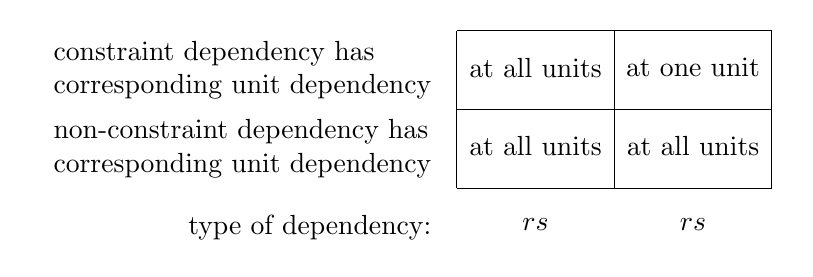
\begin{tikzpicture}
    \begin{scope}[xscale=2]
    \draw (0,0) grid (2,2);
    \node[anchor=east] at (-0.1,1.5) {\begin{tabular}{l@{}}
      constraint dependency has\\
      corresponding unit dependency~\end{tabular}};
    \node at (0.5,1.5) {\phantom{p}at all units\phantom{p}};
    \node at (1.5,1.5) {\phantom{p}at one unit\phantom{p}};

    \node[anchor=east] at (-0.1,0.5) {\begin{tabular}{l@{}}
      non-constraint dependency has\\
      corresponding unit dependency~\end{tabular}};
    \node at (0.5,0.5) {\phantom{p}at all units\phantom{p}};
    \node at (1.5,0.5) {\phantom{p}at all units\phantom{p}};

    \node[anchor=east] at (-0.1,-0.5) {type of dependency:~};
    \node at (0.5,-0.5) {\phantom{p}$r \dependsnmon s$\phantom{p}};
    \node at (1.5,-0.5) {\phantom{p}$r \dependsmon s$\phantom{p}};
    \end{scope}
  \end{tikzpicture}%
  \endpgfgraphicnamed%
  \caption{How rule dependencies are reflected in an Evaluation Graph.}
  \label{fig:constraintcovering}
\end{figure}
}%\newcommand\myfigureconstraintcovering
%
\newcommand\myfigureAtomDepGraph[1]{
  \begin{figure}[#1]%
    \centering%
    \myfigureTikzAtomDepGraph%
    \caption{Atom dependency graph of running example $\myPswim$.}
    \label{fig:swimmingatomdepgraph}
  \end{figure}
}%\myfigureAtomDepGraph
%
\newcommand\myfigureRuleDepGraph[1]{
  \begin{figure}[#1]%
    \centering%
    \myfigureTikzRuleDepGraph%
    \caption{Rule dependency graph of running example $\myPswim$.}
    \label{fig:swimmingruledepgraph}
  \end{figure}
}%\myfigureRuleDepGraph
%
%
% stopzone <- hint for vim syntax highlighting
%
\newcommand\myfigureOldEvalGraph[1]{
  %\captionsetup[subfloat]{nearskip=0pt,farskip=0pt,captionskip=0.2em}
  \begin{figure}[#1]%
    \centering%
    \myfigureExOldEvalStrat%
    \caption{Evaluation graph $\cE_1$ for running example \hex program $\myPswim$.}
    \label{fig:exOldEvalStrat}
  \end{figure}
}%\newcommand\myfigureOldEvalGraph
%
\newcommand\myfigureBetterEvalGraph[1]{
  \begin{figure}[#1]%
    \centering%
    \myfigureExBetterEvalStrat%
    \caption{Evaluation graph $\cE_2$ for running example \hex program $\myPswim$.}
    \label{fig:exBetterEvalStrat}
  \end{figure}
}%\newcommand\myfigureBetterEvalGraph
%
%
\newcommand\myfigureModelGraphOldStrat[1]{
  %\captionsetup[subfloat]{nearskip=0pt,farskip=0pt,captionskip=0.2em}
  \begin{figure}[#1]%
    \centering%
    \myfigureExOldEvalModel%
    \caption{Interpretation graph $\cI_1$ for $\cE_1$}
    \label{fig:exModelGraphOldStrat}%
  \end{figure}
}%\myfigureModelGraphOldStrat
%
\newcommand\myfigureModelGraphBetterStrat[1]{
  %\captionsetup[subfloat]{nearskip=0pt,farskip=0pt,captionskip=0.2em}
  \begin{figure}[#1]%
    \centering%
	\resizebox{\textwidth}{!}{
    \myfigureExBetterEvalModel%
	}
    \caption{Interpretation graph $\cI_2$ for $\cE_2$}
    \label{fig:exModelGraphBetterStrat}%
  \end{figure}
}%\myfigureModelGraphOldStrat
%
%
\newcommand\myfigureAlgoBuildAnswerSets[1]{%
  %\def\minskip{\vspace*{-4mm}}
  %\SetAlgoSkip{minskip}
  \begin{algorithm}[#1]
    %\begin{minipage}{10cm}
    %: creates the model graph for $\cE$
    \caption{\myBuildAnswerSets}%($\cE=(V,E)$: evaluation graph)
    \label{alg:buildAnswerSets}
    \DontPrintSemicolon
    \SetAlgoVlined
    \SetVlineSkip{1mm}
    \SetCommentSty{footnotesize}

    \KwIn{$\cE=(V,E)$: evaluation graph for \hex program $P$,
          which contains a unit $\ufinal$ that depends on all other units in $V$}
    \KwOut{a set of all answer sets of $P$}
    %
    $M := \emptyset$,
    $F := \emptyset$,
    $\myunit := \emptyset$, 
    $\mytype := \emptyset$,
    $\myint := \emptyset$,
    $U := V$ \;
    %
\smallskip

    \nlset{(a)}\label{step:whileloop}%
    \While{$U \neq \emptyset$}{
      %
      choose $u \in U$ s.t.\ $\myinputs(u) \cap U = \emptyset$ \;
      %
      let $\{ u_1,\ldots,u_k \} = \myinputs(u)$\;
      %
      \eIf{$k = 0$}{%
        %
        \nlset{(b)}\label{step:emptyinputmodels}%
        $m := \mi{max}(M) + 1$ \;
        %
        $M := M \cup \{m\}$ \;
        %
        $\myunit(m) := u$,
        %
        $\mytype(m) := \scI$,
        %
        $\myint(m) := \emptyset$\;
        %
      }{%
        %
        \nlset{(c)}\label{step:firstforloop}%
        \For{$m_1 \in \myomodels(u_1),\dotsc, m_k \in \myomodels(u_k)$}{%
          %
          \If{$J = m_1 \join \dotsb \join m_k$ is defined}{%
            %
            $m := \mi{max}(M) + 1$ \;
            %
            $M := M \cup \{m\}$,
            %
            $F := F \cup \{ (m,m_i) \mid 1\leq i\leq k \}$ \;
            %
            $\myunit(m) := u$,
            %
            $\mytype(m) := \scI$,
            %
            $\myint(m) := J$ \;
          }%
        }
      }
      %
      \nlset{(d)}\label{step:return}%
      \If{$u = \ufinal$}{%
        %
        \Return{$\myimodels(\ufinal)$} \;
      }
      %
      \nlset{(e)}\label{step:secondforloop}%
      \For{$m' \in \myimodels(u)$}{%
        %
        $O := \EvaluateLDESafe(u, \myint(m'))$ \;
        %
        \For{$o \in O$}{%
          %
          $m := \mi{max}(M) + 1$ \;
          %
          $M := M \cup \{m\}$,
          %
          $F := F \cup \{ (m,m') \}$ \;
          %
          $\myunit(m) := u$,
          %
          $\mytype(m) := \scO$,
          %
          $\myint(m) := o$ \;
        }%
      }%
      %
      \nlset{(f)}\label{step:removeu}%
      $U := U \setminus \{ u \}$ \;
    }
    %\end{minipage}
  \end{algorithm}
}% \newcommand\myfigureAlgoBuildAnswerSets[1]
%
\newcommand\myfigureAlgoEvaluateUnitOld[1]{%
  \SetAlgoSkip{}
  \begin{algorithm}[t]
    % Evaluating a unit
    \caption{$\myevaluateUnit(P\text{: \hex program}, I\text{: \hex interpretation})$}
    \label{alg:evaluateUnit}
    \DontPrintSemicolon
    \SetAlgoVlined
    \SetVlineSkip{0mm}
    \SetCommentSty{footnotesize}

    %\KwIn{$u$: evaluation unit, $m$: input model at $u$} %
    \KwOut{answer sets of $P \cup \facts(I)$ without $I$}%
    %

\smallskip

  %  \ForEach{$I\in M$}{
      %
      \tcp{determine non-disjunctive facts in $P$ and $I$}
      %
      $F := I \cups \{ a \mid r \in P \text{ such that }
                              H(r) = \{ a \} \text{ and } B(r) = \emptyset \big\}$ \;
      %
      \tcp{determine external atoms that get input only from $F$}
      %
      $\begin{array}{@{}l@{\ }l@{}}
        A_{\mi{in}} := \big\{
          \ext{g}{\vec{x}}{\vec{y}} \in r \mid
          r \in P \text{ and } & \text{for every } r' \in P
          \text{ such that } 
          \ext{g}{\vec{x}}{\vec{y}} \dependsext b \\
        & \text{it holds that } b \in F \big\}
       \end{array}$ \;
      %
      \tcp{evaluate external atom semantics and create corresponding ground replacement atoms}
      %
      $\begin{array}{@{}l@{\ }l@{}}
        I_{\mi{aux}} := \big\{
          \rat{g}(\vec{x},\vec{z}) \ {\mid}
        & \ext{g}{\vec{x}}{\vec{y}} \in A_{\mi{in}} \text{ with }
            \vec{x} = (x_1,\ldots,x_k) \text{, signature $t_i$,}\\
        & 1 \leq i \leq k,\ \vec{z} \in \extFun{g}(\Pi_{t_1}(F),\ldots,\Pi_{t_k}(F))
          \text{, and } \vec{z} \sim \vec{y} \big\}
       \end{array}$ \;
      %
     % $m' := m \cup m_{\mi{aux}}$ \;
      %
      $P' := P$ with external atoms $\ext{g}{\vec{x}}{\vec{y}} \in A_{\mi{in}}$
        replaced by auxiliaries $\rat{g}(\vec{x},\vec{y})$ \;
      %
      %choose $\mi{ES} \in \{ \textsc{Plain}, \textsc{WellF}, \textsc{GnC} \}$ according to the structure of $u'$ \;
      %
      %
      %
      %$M := \mi{ES}(u',m')$  \;%
      %
   % }
    %
    \Return{$\{ I' \setminus (I \cup I_{\mi{aux}}) \mid
                I' \in \myevaluatePregroundable(P',I \cup I_{\mi{aux}})\}$}\;
  \end{algorithm}
}%\newcommand\myfigureAlgoEvaluateUnitOld[1]
%
\newcommand\myfigureAlgoEvaluateLDESafe[1]{%
  \begin{algorithm}[#1]
  \caption{\EvaluateLDESafe}
  \label{alg:EvaluateLDESafe}
  \DontPrintSemicolon

  \KwIn{A liberally de-safe \hex{}-program $P$, an input interpretation $I$}
  \KwOut{All answer sets of $P \cup \mathit{facts}(I)$ without $I$}

%  \tcp*[h]{add input facts and ground the program}\;
%  \tcp*[h]{(cf.~\cite{eite-etal-14a})}\;
  \tcp*[h]{add input facts and ground, cf.~\cite{eite-etal-14a}}\;
  $P' \leftarrow \GroundLiberallyDomainExpansionSafeProgram(P \cup \mathit{facts}(I))$\;

  \tcp*[h]{evaluate the ground program, cf.~\cite{efkrs2014-jair},}\;
  \tcp*[h]{and perform output projection}\;
  %\Return $\big\{ I' \setminus I \cup \{ \F a \in I' \} \mid I' \in \EvaluateGroundHEX(P') \big\}$\;
  \Return $\big\{ I' \setminus I \mid I' \in \EvaluateGroundHEX(P') \big\}$\;
  \end{algorithm}%
}%\newcommand\myfigureAlgoEvaluateLDESafe[1]
%
\newcommand\myfigureAlgoGetNextUnitModel[1]{%
  \begin{algorithm}[#1]%
    %: creates the model graph for $\cE$
    \caption{$\myGetNextUnitModel(u,m_{in},m_{lastout})$}
    \label{alg:getNextUnitModel}
    \DontPrintSemicolon
    \SetAlgoVlined
    \SetVlineSkip{1mm}
    \SetCommentSty{small}
    %
    \KwIn{$u$: unit, $m_{lastout}$: omodel at $u$ or $\undef$}
    \KwOut{$m_{out}$: next omodel at $u$ (wrt.\ $m_{in}$ and $m_{lastout}$) or $\undef$}
    %
    %\tcc*{assumption: answer sets of $u$ can be calculated in fixed but arbitrary order}
    %

\smallskip

    \If{$m_{lastout} = \undef$}%
    {
      \Return{first answer set in $\AS(u \cup \facts(m_{in}))$}\;
    }{%
      $m_{out} := \text{next answer set in $\AS(u \cup \facts(m_{in}))$ after $m_{lastout}$}$\;
      %
      \lIf{$m_{out}$ exists}{%
        \Return{$m_{out}$}\;
      }%
      \lElse{%
        \Return{$\undef$}\;
      }%
    }%
  \end{algorithm}%
}% \newcommand\myfigureAlgoGetNextUnitModel[1]
%
%stopzone
%
\newcommand\myfigureAlgoGetNextIModel[1]{%
  \begin{algorithm}[#1]
    \caption{$\myGetNextIModel(u)$}
    \label{alg:getNextIModel}
    \DontPrintSemicolon
    \SetAlgoVlined
    \SetVlineSkip{1mm}
    \SetCommentSty{small}
    %
    \KwIn{$u$: unit}
    \KwOut{$m_{out}$: imodel at $u$ or $\undef$}
    %

\smallskip

    \nlset{(a)}\label{step:gnimLeaf}%
    \If{$\myinputs(u) = \emptyset$}{%
      %
      \uIf{$\mycuri(u) = \undef$}{%
        %
        \nlset{($+$)}%
        add imodel $\emptyset$ at $u$ to $\cA$\;
        %
        \Return{$\emptyset$}\;
      }
      %
      \lElse{%
        %
        \Return{$\undef$}\;
        %
        %\nlset{($-$)}%
        %remove $\mycuri(u)$ from $\cA$\;
        %
      }%
    }
    %
    let $\{ u_1,\ldots,u_k \} = \myinputs(u)$
    \tcc*{assume this order is fixed for each unit $u$}
    %
    \uIf{$\mycuri(u) \neq \undef$}{%
      %
      %%%$\mycuri(u) := \undef$\;
      %
      %\nlset{($-$)}%
      %remove $\mycuri(u)$ from $\cA$\;
      %
      $at := \myEnsureModelIncrement(u,1)$\;
      %
      \lIf{$at = \undef$}{\Return{$\undef$}}\;
      %
      $at := at - 1$\;
    }%
    \lElse{$at := k$}\;
    %
    %\tcc{\quo{$at$} keeps track which part of the join we are advancing in the loop}
    %
    \nlset{(b)}\label{step:gnimWhile}%
    \While{$at \neq 0$}{
      %
      % invariant (true at loop body begin and at loop body end, even if at = 0):
      %
      % \mycuri(u_{at+1}) ... \mycuri(u_{k})
      %         are set, are refcounted, and have common ancestor
      % \mycuri(u_j), 1 \leq j <= at
      %         may be undef or with common ancestor and are not refcounted
      %
      \uIf{$\mycuro(u_{at}) \neq \undef$}{%
        %
        %\nlset{($\vartriangle$)}%
        $\myrefcounto(u_{at}) := \myrefcounto(u_{at}) + 1$\;
        %
        $at := at - 1$\;
      }
      %
      \Else{%
        %
        $m := \myGetNextOModel(u_{at})$\;
        %
        \uIf{$m = \undef$}{%
          %
          \lIf{$at \eqs k$}{\Return{$\undef$}}\;
          %
          $at := \myEnsureModelIncrement(u,at+1)$\;
          %
          \lIf{$at = \undef$}{\Return{$\undef$}}\;
        }%
        %
        \Else{%
          %
          %\nlset{($\vartriangle$)}%
          $\myrefcounto(u_{at}) := \myrefcounto(u_{at}) + 1$\;
          %
          $at := at - 1$\;
        }
      }
    }
    %
    let $m = \mycuro(u_1) \join \cdots \join \mycuro(u_k)$\;
    %
    \nlset{($+$)}%
    add imodel $m$ to $\cA$ with dependencies to $\mycuro(u_1),\ldots,\mycuro(u_k)$\;
    %
    \Return{$m$}\;
  \end{algorithm}
}% \newcommand\myfigureAlgoGetNextIModel[1]
%
\newcommand\myfigureAlgoEnsureModelIncrement[1]{%
  \begin{algorithm}[#1]
    \caption{$\myEnsureModelIncrement(u,at)$}
    \label{alg:ensureModelIncrement}
    \DontPrintSemicolon
    \SetAlgoVlined
    \SetVlineSkip{1mm}
    \SetCommentSty{small}
    %
    \KwIn{$u$: unit with $\{u_1,\ldots,u_k\} = \myinputs(u)$, $at$: index $1 \leq at \leq k$}
    \KwOut{$at'$: index $at \leq at' \leq k$ or $\undef$}
    %

\smallskip

    \Repeat{$at = k+1$}{%
      %
      %\nlset{($\vartriangle$)}%
      $\myrefcounto(u_{at}) := \myrefcounto(u_{at}) - 1$\;
      %
      $m := \myGetNextOModel(u_{at})$\;
      %
      \lIf{$m = \undef$}{%
        %
        $at := at + 1$\;
      }%
      \Else{%
        %
        %\nlset{($\vartriangle$)}%
        $\myrefcounto(u_{at}) := \myrefcounto(u_{at}) + 1$\;
        %
        \Return{$at$}\;
      }
    }
    \Return{$\undef$}\;
  \end{algorithm}
}% \newcommand\myfigureAlgoEnsureModelIncrement[1]
%
\newcommand\myfigureAlgoGetNextOModel[1]{%
  \begin{algorithm}[#1]
    \caption{$\myGetNextOModel(u)$}
    \label{alg:getNextOModel}
    \DontPrintSemicolon
    \SetAlgoVlined
    \SetVlineSkip{1mm}
    \SetCommentSty{small}
    %
    \KwIn{$u$: unit}
    \KwOut{$m_{out}$: next omodel at $u$ or $\undef$}
    %
    %\nlset{($\vartriangle$)}%

\smallskip

    \lIf{$\myrefcounto(u) > 0$}{\Return{\undef}}\;
    %
    \lIf{$\mycuri(u) = \undef$}{$\mycuri(u) := \myGetNextIModel(u)$}\;
    %
\nop{*********** hide *******
    \While{$\mycuri(u) \neq \undef$}{%
      % true here: \mycuri(u) != \undef
      % true here: \mycuro(u) = \undef or (\mycuro(u),\mycuri(u)) \in F
      %
      \nlset{(!!!)}%
      $m_{last\scO} := \mycuro(u)$\;
      %
      \nlset{(!!!)}%
      $\mycuro(u) := \myGetNextUnitModel(u,\mycuri(u),m_{last\scO})$\;
      %
      %\nlset{($-$)}%
      %\lIf{$m_{last\scO} \neq \undef$}{%
      %  %
      %  remove $m_{lastout}$ from $\cA$\;
      %}
      %
      \If{$\mycuro(u) \neq \undef$}{%
        %
        \nlset{($+$)}%
        add omodel $\mycuro(u)$ to $\cA$ with dependency to $\mycuri(u)$\;
        %
        \Return{$\mycuro(u)$}\;
      }
      %
      $\myGetNextIModel(u)$\;
      %
    }
    \nlset{(replacement?)}%
    \While{$\mycuri(u) \neq \undef$}{%
      % true here: \mycuri(u) != \undef
      % true here: \mycuro(u) = \undef or (\mycuro(u),\mycuri(u)) \in F
      %
      \uIf{$\mycuro(u) = \undef$}{%
        $\mycuro(u) := $ the first answer set in $\AS(u \cups \facts(\mycuri(u)))$\;
      }%
      \lElse{%
        $\mycuro(u) := $ the answer set in $\AS(u \cups \facts(\mycuri(u)))$ after $\mycuro(u)$\;
      }%
      \uIf{such an answer set $\mycuro(u)$ does not exist}{%
        $\mycuro(u) := \undef$
      }%
      \Else{%
        %
        \nlset{($+$)}%
        add omodel $\mycuro(u)$ to $\cA$ with dependency to $\mycuri(u)$\;
        %
        \Return{$\mycuro(u)$}\;
      }
      %
      $\myGetNextIModel(u)$\;
      %
    }
******************* hide *************}
    %\nlset{(TE: replacement suggestion)}%
    \While{$\mycuri(u) \neq \undef$}{%
      % true here: \mycuri(u) != \undef
      % true here: \mycuro(u) = \undef or (\mycuro(u),\mycuri(u)) \in F
      %
%      \lIf{$\mycuro(u) = \undef$}{$n := 0$} \lElse{$n := n+1$}\;
%      $\mycuro(u) := \myNextAnswerSet(u \cups \facts(\mycuri(u)),n)$\;
      $\mycuro(u) := \myNextAnswerSet(u \cups \facts(\mycuri(u)),\mycuro(u))$\;
      \If{$\mycuro(u) \neq \undef$}{%
        %
        \nlset{($+$)}%
        add omodel $\mycuro(u)$ to $\cA$ with dependency to $\mycuri(u)$\;
        %
        \Return{$\mycuro(u)$}\;
      }
      %
      $\mycuri(u) := \myGetNextIModel(u)$\;
      %
    }
    \Return{$\undef$}\;
  \end{algorithm}
}% \newcommand\myfigureAlgoGetNextOModel[1]
%
%
% stopzone %
%
\newcommand\myfigureAlgoGetNextIModelOld[1]{%
  \begin{algorithm}[#1]
    \caption{$\myGetNextIModel(u,m_{\mi{lastin}})$}
    \label{alg:getNextIModel}
    \DontPrintSemicolon
    \SetAlgoVlined
    \SetVlineSkip{1mm}
    \SetCommentSty{small}
    %
    \KwIn{$u$: unit, $m_{lastin}$: imodel at $u$ or $\undef$}
    \KwOut{$m_{out}$: imodel at $u$ or $\undef$}
    %
\smallskip

    \nlset{(a)}\label{step:gnimLeaf}%
    \If{$\myinputs(u) = \emptyset$}{%
      %
    \lIf{$m_{lastin} = \undef$}{\Return{$\emptyset\,$}} \lElse{\Return{\undef}}
    }
    %
    let $\{ u_1,\ldots,u_k \} = \myinputs(u)$
    \tcc*{assume this order is fixed for each unit $u$}
    %
    \eIf{$m_{lastin} = \undef$}{%
      %
      $m_i := \undef$ for $1 \leq i \leq k$\;
      %
      $at := k$ \tcc*{\quo{$at$} keeps track which part of the join we are advancing in the loop}
    }{%
      %
      $m_i := m$ with $(m_{lastin},m) \in F$, $\myunit(m) = u_i$, $1 \leq i \leq k$\;
      %
      \nlset{($\star$)}%
      remove $m_{lastin}$ from $\cA$\;
      %
      $at := 1$ \tcc*{\quo{$at$} keeps track which part of the join we are advancing in the loop}
    }
    %
    \nlset{(b)}\label{step:gnimWhile}
    \While{\mb{true}}{
      % true here: \{m_{at+1},...,m_k\} have common ancestor
      %
      $m_{at} := \myGetNextOModel(u_{at},m_{at})$\;
      %
      \nlset{(c)}\label{step:gnimAfterRepeat}%
      \uIf{$m_{at} = \undef$}{%
        %
        \nlset{(d)}\label{step:gnimNoMoreJoin}%
        \lIf{$at = k$}{%
          %
          \Return{\undef}\;
        }
        \lElse{%
          %
          $at := at + 1$\;
        }
        %
      }%
      \ElseIf{$m_{at},\ldots,m_k$ have common ancestor at all $\mycau(u)$}{%
        %
        \uIf{$at = 1$}{%
          %
          let $m = m_1 \join \cdots \join m_k$\;
          %
          store new imodel $m$ with dependencies to $m_1,\ldots,m_k$\;
          %
          \Return{$m$}\;
        }
        \lElse{%
          $at := at - 1$\;
          %
        }
      }
    }
  \end{algorithm}
}% \newcommand\myfigureAlgoGetNextIModelOld[1]
%
\newcommand\myfigureAlgoGetNextOModelOld[1]{%
  \begin{algorithm}[#1]
    \caption{$\myGetNextOModel(u,m_{lastout})$}
    \label{alg:getNextOModel}
    \DontPrintSemicolon
    \SetAlgoVlined
    \SetVlineSkip{1mm}
    \SetCommentSty{small}
    %
    \KwIn{$u$: unit, $m_{lastout}$: omodel at $u$ or $\undef$}
    \KwOut{$m_{out}$: next omodel (wrt.\ $m_{lastout}$) at $u$ or $\undef$}
    %
\smallskip

    \lIf{$m_{lastout} = \undef$}%
      {$m_{in} := \myGetNextIModel(u,\undef)$}\;
    \lElse{$m_{in} := m$ s.t.\ $(m_{lastout},m) \in F$}\;
    %
    $m_{out} := m_{lastout}$\;
    %
    \While{$m_{in} \neq \undef$}{%
      % true here: m_{in} != \undef
      % true here: m_{out} = \undef or (m_{out},m_{lastin}) \in F 
      %
      $m_{out} := \myGetNextUnitModel(u,m_{in},m_{out})$\;
      %
      \nlset{($\star$)}%
      \If{$m_{lastout} \neq \undef$}{%
        %
        remove $m_{lastout}$ from $\cA$\;
        %
        $m_{lastout} := \undef$\;
      }
      %
      \If{$m_{out} \neq \undef$}{%
        %
        add $m_{out}$ to $\cA$ as output model with dependency to $m_{in}$\;
        %
        \Return{$m_{out}$}\;
      }
      %
      $m_{in} = \myGetNextIModel(u,m_{in})$\;
      %
    }
    \Return{$\undef$}\;
  \end{algorithm}
}% \newcommand\myfigureAlgoGetNextOModelOld[1]

\newcommand\myfigureMCStimetable{
  {
  \small
  \begin{tabular}{|c|r|r||r|r||r|r|}
  \cline{2-7}
  \multicolumn{1}{c|}{}
   & \multicolumn{2}{c||}{Average time (sec)}
   & \multicolumn{2}{c||}{Minimum time (sec)}
   & \multicolumn{2}{c|}{Maximum time (sec)} \\
  \cline{1-1}
  Instance group &
  \qquad\heurold &
  \heurnew &
  \qquad\heurold &
  \heurnew &
  \qquad\heurold &
  \heurnew \\
  \hline
  \hline
  D-7-7-3-3 &  94.7 &  0.3 &   1.9 & 0.2 & --- &   0.4 \\
  \hline
  D-7-7-4-4 & 463.5 &  0.9 &   7.0 & 0.3 & --- &   2.2 \\
  \hline
  D-7-7-5-5 &   --- &  3.1 &   --- & 0.9 & --- &  11.1 \\
  \hline
  H-9-9-3-3 &   --- &  0.9 &   --- & 0.4 & --- &   2.0 \\
  \hline
  H-9-9-4-4 &   --- & 16.2 &   --- & 0.6 & --- & 132.0 \\
  \hline
  R-7-7-4-4 &   --- &  0.9 &   --- & 0.4 & --- &   2.4 \\
  \hline
  R-7-7-5-5 &   --- &  1.8 &   --- & 0.5 & --- &   2.6 \\
  \hline
  R-7-8-5-5 & 569.5 &  2.2 & 295.2 & 0.3 & --- &   4.9 \\
  \hline
  R-7-9-5-5 &   --- &  2.0 &   --- & 0.5 & --- &   4.1 \\
  \hline
  R-8-7-5-5 &   --- &  2.7 &   --- & 0.6 & --- &   6.9 \\
  \hline
  R-8-8-5-5 &   --- &  2.3 &   --- & 0.4 & --- &   4.7 \\
  \hline
  Z-7-7-3-3 & 176.5 &  1.2 &   4.1 & 0.2 & --- &   6.8 \\
  \hline
  Z-7-7-4-4 & 513.5 &  1.5 &  69.9 & 0.5 & --- &   3.1 \\
  \hline
  Z-7-7-5-5 &   --- &  8.5 &   --- & 1.8 & --- &  44.6 \\
  \hline
  \end{tabular}
  }
}
%
\newcommand\myfigureMCSmemtable{
  {
  \small
  \begin{tabular}{|@{\;}c@{\;}|r|r||r|r||r|r|}
  \cline{2-7}
  \multicolumn{1}{c|}{}
   & \multicolumn{2}{@{\;}c@{\;}||}{Average memory (MB)}
   & \multicolumn{2}{@{\;}c@{\;}||}{Minimum memory (MB)}
   & \multicolumn{2}{@{\;}c@{\;}|}{Maximum memory (MB)} \\
  \cline{1-1}
  Instance group &
  \qquad\heurold &
  \heurnew &
  \qquad\heurold &
  \heurnew &
  \qquad\heurold &
  \heurnew \\
  \hline
  \hline
  D-7-7-3-3 &  612.3 &   7.0 &   11.1 &  4.5 & --- &   9.9 \\
  \hline
  D-7-7-4-4 & 1579.2 &  15.1 &  198.9 &  6.0 & --- &  32.0 \\
  \hline
  D-7-7-5-5 & 1714.1 &  41.2 &  413.4 & 11.3 & --- &  90.1 \\
  \hline
  H-9-9-3-3 & 1673.1 &  22.2 &  398.5 &  7.0 & --- &  59.6 \\
  \hline
  H-9-9-4-4 &    --- & 110.5 &    --- & 10.8 & --- & 332.4 \\
  \hline
  R-7-7-4-4 & 1908.2 &  18.0 &  494.0 &  7.1 & --- &  42.6 \\
  \hline
  R-7-7-5-5 &    --- &  42.5 &    --- & 10.2 & --- &  74.9 \\
  \hline
  R-7-8-5-5 & 2885.8 &  36.5 & 1910.9 &  6.9 & --- & 120.8 \\
  \hline
  R-7-9-5-5 &    --- &  34.8 &    --- &  7.2 & --- &  74.2 \\
  \hline
  R-8-7-5-5 & 2921.9 &  43.8 & 2219.2 & 10.1 & --- &  85.1 \\
  \hline
  R-8-8-5-5 &    --- &  38.4 &    --- & 14.1 & --- &  80.7 \\
  \hline
  Z-7-7-3-3 &  925.6 &  34.6 &   42.9 &  6.8 & --- & 260.5 \\
  \hline
  Z-7-7-4-4 & 1161.8 &  31.8 &  251.3 &  8.5 & --- &  89.8 \\
  \hline
  Z-7-7-5-5 & 2276.9 &  83.3 &  495.3 & 29.4 & --- & 291.8 \\
  \hline
  \end{tabular}%
  }
}
%
\newcommand{\myfigureMCStime}[1]{%
  \begin{figure}[#1]
    \centering%
    \includegraphics[width=0.9\textwidth]{dmcs_timecomparison} \\[1em]
    \myfigureMCStimetable%
    \caption{Time comparison for enumerating output-projected equilibria of MCS instances.
     Each instance group contains 10 instances,
     maximum time/memory was 600 sec/3000 MB,
     time/memory exhaustion is indicated by `---'.}
    \label{fig:mcsbenchtime}%
  \end{figure}
}%
%
\newcommand{\myfigureMCSmem}[1]{%
  \begin{figure}[#1]
    \centering%
    \includegraphics[width=0.9\textwidth]{dmcs_memcomparison} \\[1em]
    \myfigureMCSmemtable%
    \caption{Memory usage comparison for enumerating output-projected equilibria of MCS instances.
     Each instance group contains 10 instances,
     maximum time/memory was 600 sec/3000 MB,
     time/memory exhaustion is indicated by `---'.}
    \label{fig:mcsbenchmem}%
  \end{figure}
}%
%
\newcommand{\myfigureRevSelExtTable}{%
  {
  \small
  \begin{tabular}{|c||r|r||r|r|}
  \cline{2-5}
  \multicolumn{1}{c|}{}
   & \multicolumn{2}{c||}{Memory usage (MB)}
   & \multicolumn{2}{c|}{Time usage (sec)} \\
  \cline{1-1}
  $T$ &
  \heurold & \heurnew &
  \heurold & \heurnew \\
  \hline
    1 &   31.7 &   31.5 &   1.45 &  1.36 \\
  \hline
    2 &   72.7 &   56.2 &   2.65 &  2.11 \\
  \hline
    3 &  112.1 &   82.0 &   4.17 &  3.15 \\
  \hline
    4 &  142.4 &  106.3 &   5.82 &  4.02 \\
  \hline
    5 &  180.2 &  131.3 &   8.21 &  5.25 \\
  \hline
    6 &  239.6 &  165.2 &  11.92 &  6.17 \\
  \hline
    7 &  258.5 &  164.5 &  16.31 &  7.17 \\
  \hline
    8 &  309.4 &  213.7 &  28.08 &  7.92 \\
  \hline
    9 &  422.4 &  250.1 &  51.74 &  9.58 \\
  \hline
   10 &  588.3 &  242.2 & 100.26 & 10.87 \\
  \hline
   11 & 1413.7 &  262.4 & 206.24 & 12.01 \\
  \hline
   12 &    --- &  294.3 &    --- & 21.00 \\
  \hline
   20 &    --- &  444.4 &    --- & 33.45 \\
  \hline
   30 &    --- &  761.2 &    --- & 46.23 \\
  \hline
   40 &    --- & 1118.2 &    --- & 62.61 \\
  \hline
   50 &    --- & 1408.2 &    --- & 65.00 \\
  \hline
  \end{tabular}%
  }
}
%
\newcommand{\myfigureRevSelExt}[1]{%
  \begin{figure}[#1]
    \centering%
    \includegraphics[width=0.85\textwidth]{revsel_ext_time} \\[-1ex]
    \includegraphics[width=0.85\textwidth]{revsel_ext_mem} \\[1ex]
    \myfigureRevSelExtTable
    \caption{\textsc{RevSel 1} benchmark results:
     \heurold always exhausts 3000 MB memory (indicated by `---') before it times out;
     \heurnew always terminates successfully within the 600 sec time limit.}
    \label{fig:revselexttimemem}%
  \end{figure}
}%
%
\newcommand{\myfigureRevSelExtlinear}[1]{%
  \begin{figure}[#1]
    \centering%
    \includegraphics[width=0.9\textwidth]{revsel_ext_time_mem_h2} \\[1em]
    \caption{Linear plot of time and memory usage of \heurnew with \textsc{RevSel 1}:
     this shows that \heurnew scales linearly in both time and space,
     as opposed to \heurold which scales exponentially or worse.}
    \label{fig:revselextlinear}%
  \end{figure}
}%
%
\newcommand\myfigureRevSelPumpingTable{
  {
  \small
  \begin{tabular}{|c||r|r||r|r||r|r||r|r|}
  \cline{2-9}
  \multicolumn{1}{c|}{} &
  \multicolumn{2}{|c||}{\dlv} &
  \multicolumn{2}{c||}{\clingo} &
  \multicolumn{2}{c||}{\heurnew + \dlv} &
  \multicolumn{2}{c|}{\heurnew + \clingo} \\
  \cline{1-1}
  $P$ &	time &	memory &	time &	memory &	time &	memory &	time &	memory \\
  \hline
  10 &	0.45 &  	9.8 &	  0.20 &	  6.4 & 	0.47 &	  8.8 &	  0.28 &    5.3 \\
  20 &	8.57 &	230.8 &	  3.92 &	 80.6 & 	5.48 &	112.8 &	  2.99 &   18.7 \\
  30 & 36.62 &	914.9 &	 23.93 &	380.8 &  26.79 &	398.0 &	 14.61 &   70.6 \\
  40 &	---  &	  --- &	 90.33 & 1134.8 &	 83.50 &	855.4 &	 65.25 &  210.1 \\
  50 &	---  &  	--- &	262.91 & 2890.7 &	206.17 & 2061.6 &	193.36 &  497.9 \\
  60 &	---  &  	--- &	   --- &    --- &	437.47 & 2074.8 &	411.15 & 1002.4 \\
  \hline
  \end{tabular}%
  }
}
%
\newcommand{\myfigureRevSelPumping}[1]{%
  \begin{figure}[#1]
    \centering%
    \includegraphics[width=0.85\textwidth]{revsel_pumping_time_mem_dlv} \\[1em]
    \includegraphics[width=0.85\textwidth]{revsel_pumping_time_mem_clingo} \\[1em]
    \myfigureRevSelPumpingTable
    \caption{\textsc{RevSel 2} benchmark results (top \dlv, bottom \clingo):
     both solvers do not manage to solve instances above a certain size,
     however if we use \heurnew to decompose the computation, it uses less memory and time.}
    \label{fig:revselpumping}%
  \end{figure}
}%

\newcommand\myfigureAlgoOnDemandAS[1]{%
  \begin{algorithm}[#1]
    \caption{$\myOnDemandAS$}
    \label{alg:OnDemandAS}
    \DontPrintSemicolon
    \SetAlgoVlined
    \SetVlineSkip{1mm}
    \SetCommentSty{small}
    %
    \KwIn{evaluation graph $\cE$ for program $P$, with final unit $\ufinal=\emptyset$}
    \KwOut{the answer sets of $P$}
    %
\smallskip

    initialize global storage ${\cal S}$\;
    \Repeat{$m_{out} = \undef$}{%
      $m_{out}$ := \myGetNextOModel($\ufinal$)\; 
      \lIf{$m_{out} \neq \undef$}{output $m_{out}$}
      }
\label{MyAlgOnDemandAS}
  \end{algorithm}
}% \newcommand\myfigureAlgoGetNextOModelOld[1]
